\documentclass[11pt, a4paper]{article}

\usepackage{amsmath}
\usepackage{amsfonts} %Matheschriften
\usepackage{amssymb} %Mathesymbole
%\usepackage{mathptmx} % Einstellung für Schriften und Sonderzeichen in mathematischen Umgebungen
                        % ändert SChriftfont
\usepackage{wasysym} % Stellt diverse Sonderzeichen bereit
\usepackage{siunitx}
\usepackage{float}
\usepackage{microtype}
\usepackage{graphicx}
\usepackage{hyperref}
\usepackage{xcolor}
\usepackage[section]{placeins}
% allows for temporary adjustment of side margins
\usepackage{changepage}
\usepackage{rotating}
\usepackage{tikz}
\usepackage{circuitikz}


\usepackage[ngerman]{babel}
\addto\captionsngerman{%
 \renewcommand{\abstractname}{Einleitung}}

\title{Versuch 2: Brückenschaltung}
\author{Team 2-13: Jascha Fricker, Benedict Brouwer}

\begin{document}
    \maketitle

    \tableofcontents

    \newpage

    \section{Einleitung}
    Durch die wheatonsche Brückenschaltung können Widerstände und Impedanzen sehr genau bestimmt werden. In diesem Versuch werden mit dieser Methode verschiedene, Widerstände, Spulen und Kondensatoren untersucht.
    \section{Experimenteller Aufbau}
    \begin{circuitikz}
        \ctikzset{european resistors}
        \draw (0,0)
        to[V,v=$U_q$] (0,4) % The voltage source
        to[short] (2,4)
        to[R=$Z_1$] (2,2) % The resistor
        to[R=$Z_2$] (2,0) % The resistor
        to[short] (0,0);
        \draw (2,0)
        to[short] (6,0)
        to[pR=$1k\si{\ohm}$] (6,4)
        to[short] (2,4);
        \draw (2,2)
        to[ammeter] (5.5,2);
        \label{circuit}
     \end{circuitikz}
    \section{Theorie}
    In diesem Versuch werden mithilfe der in \ref{circuit} gezeigten Brückenschaltung verschiedene Widerstände, Spulen und Kondensatoren untersucht.
    Wenn kein Strom durch das Ampèremeter fließt, bzw. die lissajous Kurve auf dem Oszilloskop die Form einer horizontalen Linie animmt, gilt die Schaltung als abgeglichen und es gilt das Verhältnis
    \begin{align}
        \frac{Z_1}{Z_2} = \frac{R_3}{R_4} = \frac{R_p}{1\si{\kilo\ohm} - R_p} \\
        \Rightarrow Z_1 = \frac{R_p}{1\si{\kilo\ohm} - R_p} \cdot Z_2 \,,
    \end{align}
    wobei $R_p$ der Ablesewert des Potentiometers ist, und $Z_2$ der bekannte (komplexe) Vergleichswiderstand.

    Wenn eine Spule gemessen wird, gilt speziell
    \begin{align}
        R_1 &= \frac{R_P}{1\si{\kilo\ohm} - R_P} \cdot \left(R_S + R_V\right) \\
        L_1 &= \frac{R_P}{1\si{\kilo\ohm} - R_P} \cdot \left(L_S\right) \\
        \text{mit} \ \ Z_2 &= R_2 + j\omega L_2 = R_V + R_S + j\omega L_S \,,
    \end{align}
    wobei $R_S$ der bekannte Widerstand, $L_S$ die bekannte Induktivität der Spule und $R_V$ der Wert des zweiten (kleinen) Potentiometers ist, welcher in Reihe mit der bekannten Spule geschaltet wurde.

    Wenn ein Kondensator gemessen wird, gilt analog mit $R_1 = 0$
    \begin{align}
        \frac{Z_1}{Z_2} = \frac{\frac{1}{i \omega C_1}}{R_2 + \frac{1}{i \omega C_2}} \overset{Im \, = \, 0}{=} \frac{1}{\omega^2 \cdot C_1 C_2} \cdot \frac{1}{R_2^2 + \frac{1}{\omega^2 C_2^2}} = \frac{R_p}{1\si{\kilo\ohm} - R_p} \\
        \overset{Umstellen \ nach \ C_1}{\Rightarrow} \ \ C_1 = \frac{1 \si{\kilo\ohm} - R_P}{R_P} \cdot \frac{1}{\omega^2 R_2^2 C_2^2 + 1}\cdot C_2 \,,
    \end{align}
    wobei $C_2$ die Kapazität des bekannten Kondensator ist.
    \section{Ergebnisse und Diskussion}
    \paragraph{Aufgabe 7}
    Durch das Potentiometer kann für jeden der 3 Vorwiderstände der Widerstand des maximal eingestellten Potentiometer bestimmt werden. Die Ergebnisse sind in Tabelle \ref{tab:./BRU/wiepo} aufgeführt. Zu erkennen ist, dass der bei $10 \si{\ohm}$ errechnete Widerstand sehr start abweicht, während bei $30 \si{\ohm}$ und $100 \si{\ohm}$ sehr genau zum angegebenen Wert von $100 \si{\ohm}$ passen Dies könnte daran liegen, dass die Brückenschaltung bei sehr verschiedenen $R_1$ und $R_2$ nicht sehr genau ist.
    \input{wiepo.txt}

    \paragraph{Aufgabe 8}
    Hier wurden die reellen Widerstände der verschiedenen Spulen gemessen. Die Ergebnisse sind in Tabelle \ref{tab:./BRU/wiespu} aufgeführt. Auf den Spulen waren leider keine Werte angegeben. Die Werte der großen Spule sind aber in sich relativ konsistent, da die zwei Messungen mit dem Mittelabgriff M ungefähr halb so groß wie der Widerstand der gesamten Spule sind.

    \input{wiespu.txt}

    \paragraph{Aufgabe 9 und 10}
    Die Messwerte dieser Aufgaben können im Anhang \ref{tab:./BRU/eigglueh} gefunden werden. In Graph \ref{amp} wurde die Beziehung zwischen Stromstärke und Widerstand aufgetragen. In Graph \ref{pow} jene zwischen Leistung ung Widerstand. Wie zu erwarten, ist der Widerstand nicht ohmsch, sondern steigt bei größerer Stromstärke / Leistung an. Deshalb stimmen die Werte auch trotz ihren Unsicherheitsbereiches nicht überein. Der Widerstand steigt, da die Glühlampe zu leuchten beginnt und Energie durch Licht abgibt.

    \begin{figure}
        \centering
        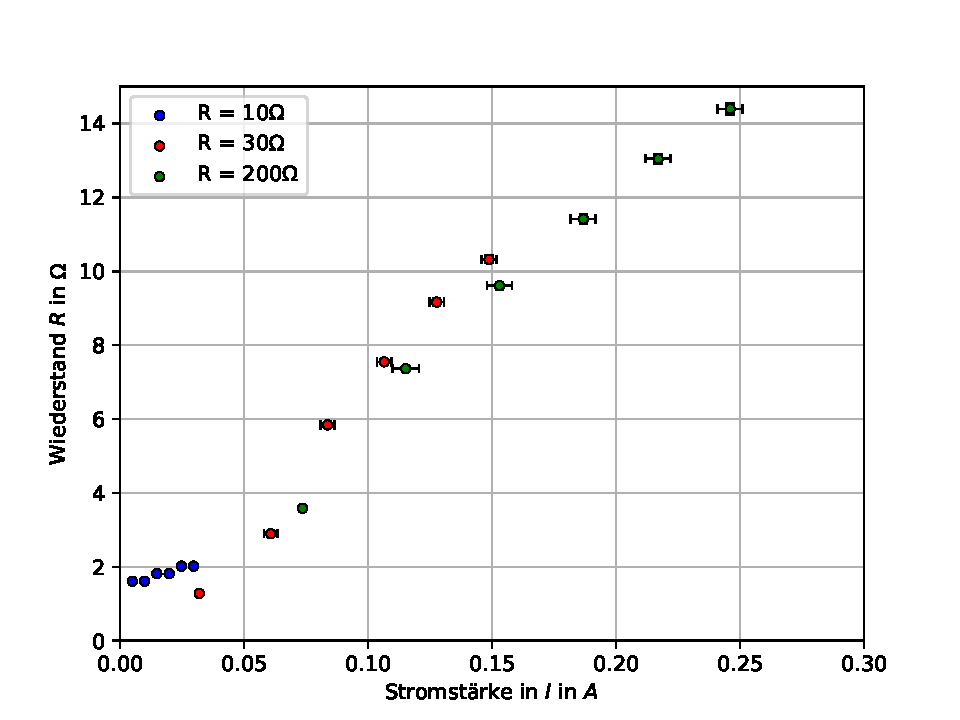
\includegraphics[width=\textwidth]{amp.pdf}
        \caption{Beziehung zwischen Stromstärke und Widerstand}
        \label{amp}
    \end{figure}
    \begin{figure}
        \centering
        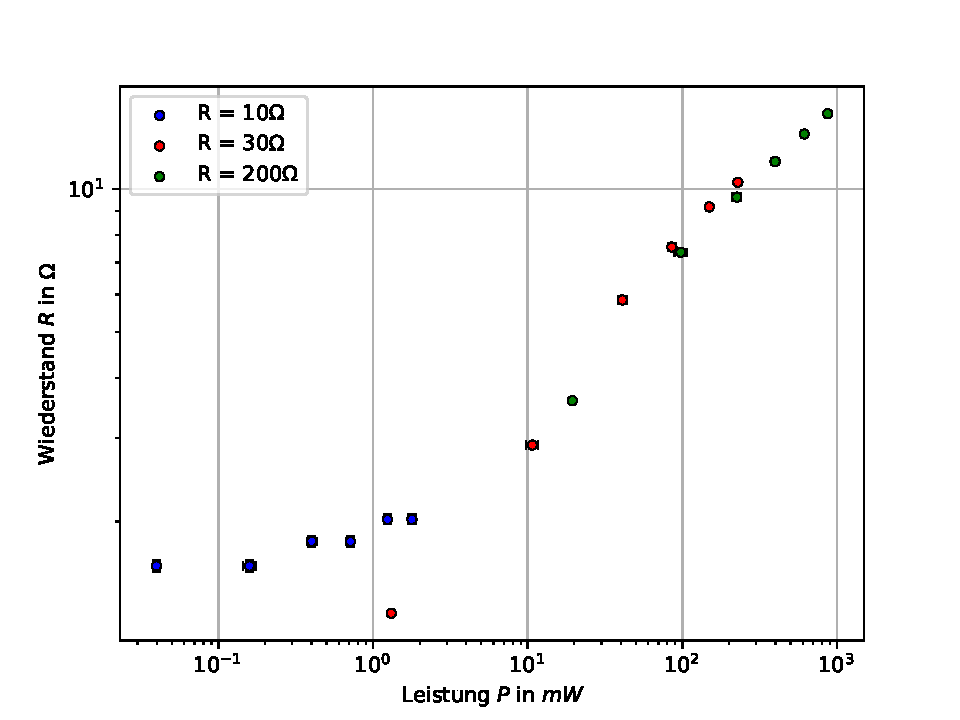
\includegraphics[width=\textwidth]{pow.pdf}
        \caption{Beziehung zwischen Leistung und Widerstand}
        \label{pow}
    \end{figure}

    \paragraph{Aufgabe 11}
    In der Tabelle \ref{tab:./BRU/komp} sind die Messwerte und Ergebnisse für die verschiedenen Spulen aufgeführt. Es wurden beide Spulen mit beiden unbekannte Spulen gemessen. Approximiert man die Spule als lange Spule gilt
    \begin{align}
        L &= \mu_0 \frac{A\cdot N^2}{l} \\
        \Rightarrow \ \ L_{1/2} &= mu_0 \frac{A\cdot \left(\frac{N}{2}\right)^2}{l} = \frac{1}{4} \cdot L \,. \label{lspu}
    \end{align}
    Es kann erkannt werden, dass die Wert des beiden Spulen zwar jewels bei einer Vergleichsspule übereinstimmen, aber insgesamt sehr unterschiedich sind. Wir wissen nicht, woran das liegt.

    \input{komp.txt}

    \paragraph{Aufgabe 13}
    Auch die Kapazitäten der unbekannten Kondensatoren konnten bei einer Frequenz von $\omega = 1000(10) \si{\kilo\hertz}$ und einem Vergleichkondensator mit $C_2 = 1.00(5) \si{\micro\farad}$ ermittel werden. Diese werden in \ref{tab:./BRU/kond} aufgelistet. Wie bei Aufgabe 11 können hier mangels Literaturwerten keine Aussagen zur Richtigkeit gemacht werden.
    
    \input{kond.txt}

    \section{Fazit}
    Durch die Experimente wurde gezeigt, wie man sowohl relle als auch komplexe Widerstände durch die Brückenschaltung bestimmen kann. Bis auf die Spule (bezugnehmend auf Afgabe 11) sind eigentlich alle anderen Werte in sich konsistent, wären wir dort aber der Aufgabenstellung gefolgt, und hätten nur mit einer Spule gemessen, wäre diese Diskrepanz nicht aufgefallen - manchmal ist es gut, zur Sicherheit mehr Werte zu messen. Vor allem die Messung der nicht-ohmschen Glühlampe ist aus physikalischer Sicht interessant.

    \section{Anhang}
    \subsection{Gaußsche Fehlerfortpflanzung}
    Die Fehlerfortpflanzung wurde mithilfe der Formel
    \begin{align}
        u\left(g \left(x_1, ..., x_n\right)\right) = \sqrt{\sum_{i=1}^n \left( \frac{\partial g }{\partial x_i} \cdot u\left(x_i\right) \right)^2} \label{gauss}
    \end{align}
    berechnet.
    \subsection{Messwerte Aufgabe 9 und 10}
    \input{eigglueh.txt}

    \bibliographystyle{plain}
    \bibliography{literature}

\end{document}